
% Let a rigid body have positional coordinates $q^{i}$, and momentum $p_{i}$. By the 15th century CE, Fermat discovered the least path principle for light, which dictates that light will always travel on a path such that its travel time is a local minimum in the space of possible paths. This principle explained Snell's law, which states for two media with indices of refraction $\beta_{1}$ and $\beta_{2}$, a light ray striking the $\beta_{1}$-indexed material at an angle $\theta_{1}$ from the normal will scatter at an angle $\theta_{2}$. The scattering angle $\theta_{2}$ is determined by the three parameters $\beta_{1}$, $\theta_{1}$ and $\beta_{2}$ via $\beta_{1} \sin \theta_{1} = \beta_{2} \sin \theta_{2}$.

% This principle was generalized to Lagrange's Principle, which states that for a mechanical system we can construct a scalar function $\mathcal{L}(q^{i}, \dot{q}^{i})$ called the Lagrangian, such that its integral is stationary in the space of possible paths. Call this integral the action: $S = \int_{\eta(t)} \mathcal{L} dt$. The path $\eta$ is the same as the path that Newton's laws would have dictated in the absence of external forces.
% \begin{equation}
% \delta S = \delta \left[ \int_{\eta(t)} \mathcal{L} dt \right] = 0
% \end{equation}
% \begin{figure}[htbp]
%     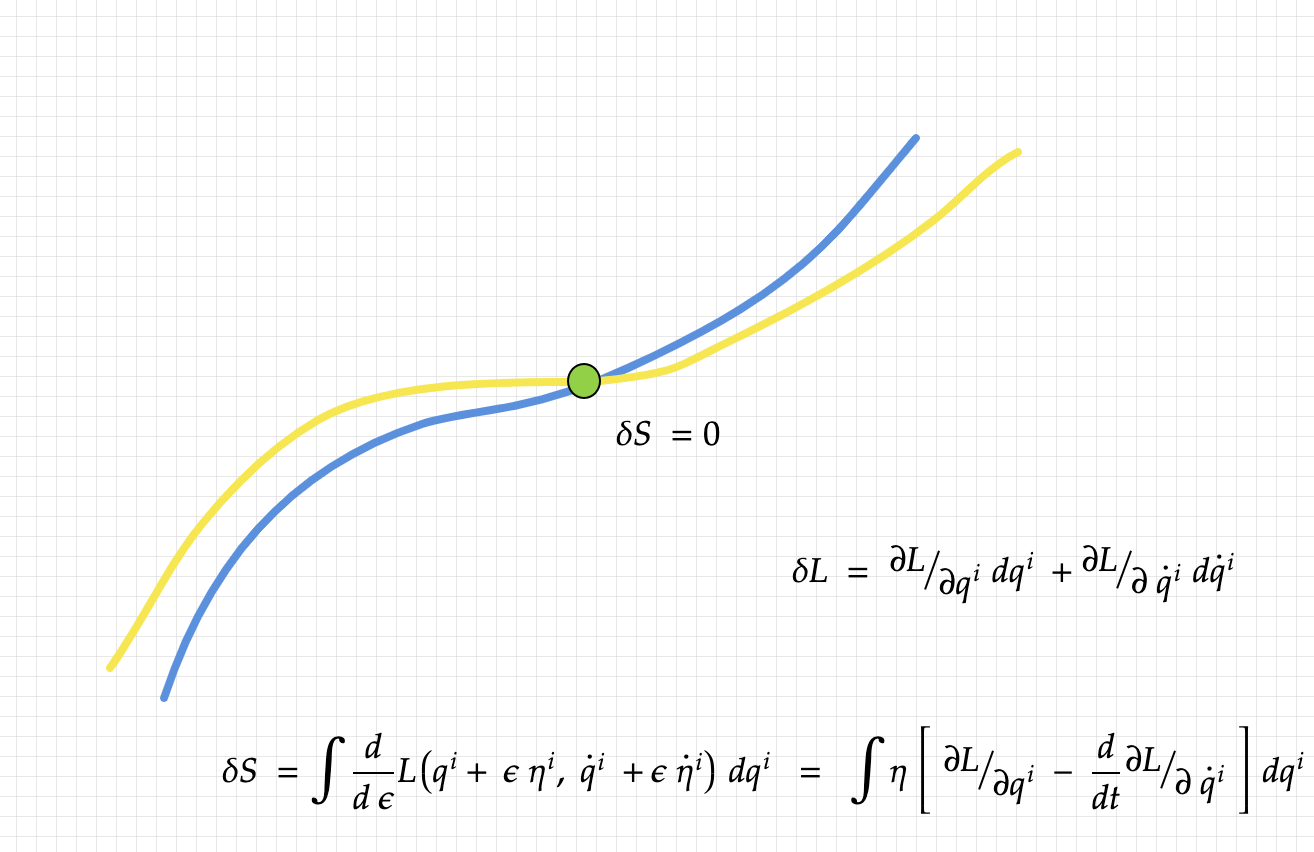
\includegraphics[width=1.0\linewidth]{Chapters/Figures/Screenshot 2025-02-21 at 7.59.09 AM.png}
%     \caption{An illustration of how one can compute $\delta S$ using first principles. Considering a perturbation of the path $q^{i}$ by $\epsilon \eta$, and taking a derivative with respect to $\epsilon$.}
%     \label{fig:compute_delta_S}
% \end{figure}
% The variation is considered to be a smooth perturbation of $q^{i}$ according to a smooth deformation of $q^{i}$ into path $\eta$, with weight $\epsilon$ as $\epsilon \to 0$. Passing the variation to the inside and integrating by parts, we have:
% \begin{equation}
% \left[ \int_{\eta(t)} \left( \frac{\partial \mathcal{L}}{\partial q^{i}} - \frac{d}{dt} \frac{\partial \mathcal{L}}{\partial \dot{q}^{i}} \right) \eta dt \right] = 0
% \end{equation}
% One may show $\mathcal{L}$ satisfies the following differential equation:
% \begin{equation}
% \frac{\partial \mathcal{L}}{\partial q^{i}} - \frac{d}{dt} \frac{\partial \mathcal{L}}{\partial \dot{q}^{i}} = 0
% \end{equation}
% Assume we are working with uniqueness to solutions of differential equations. Then, if we find a solution to this differential equation, which we call the Lagrangian, we know that for a proposed path of motion, this is the scalar we will integrate over time on our path. If the integration of the scalar on a path, as compared to its neighbors, produces a local minimum, the path will be taken by the particle. Now, for a moment there is something important to mention. 
